\documentclass[conference]{IEEEtran}
\IEEEoverridecommandlockouts

\usepackage[utf8]{inputenc}
\usepackage[T1]{fontenc}
\usepackage[english]{babel}
\usepackage{cite}
\usepackage{amsmath,amssymb,amsfonts}
\usepackage{graphicx}
\usepackage{textcomp}
\usepackage{xcolor}
\usepackage{booktabs}
\usepackage{array}
\usepackage{url}
\usepackage{hyperref}
\usepackage{tikz}
\usetikzlibrary{positioning, fit, arrows.meta, backgrounds}

\def\BibTeX{{\rm B\kern-.05em{\sc i\kern-.025em b}\kern-.08em
    T\kern-.1667em\lower.7ex\hbox{E}\kern-.125emX}}

% ──────────────────────────────────────────────────────────────────────────────
\begin{document}

\title{ContAR: A No-Code WebAR Authoring Platform\\
for 3D Virtual Narrators in Anti-Racist Education}

\author{
  \IEEEauthorblockN{Jorge Luiz Cunha de Freitas}
  \IEEEauthorblockA{
    \textit{Centro de Informática (CIn)}\\
    \textit{Universidade Federal de Pernambuco (UFPE)}\\
    Recife, Brazil\\
    jlf@cin.ufpe.br
  }
  \and
  \IEEEauthorblockN{Manoela Milena Oliveira da Silva}
  \IEEEauthorblockA{
    \textit{Centro de Informática (CIn)}\\
    \textit{Universidade Federal de Pernambuco (UFPE)}\\
    Recife, Brazil\\
    mmos@cin.ufpe.br
  }
  \and
  \IEEEauthorblockN{Guilherme José Ferreira de Araújo}
  \IEEEauthorblockA{
    \textit{Universidade de Pernambuco (UPE)}\\
    Petrolina, Brazil\\
    guilherme.jose@upe.br
  }
  \and
  \IEEEauthorblockN{Francisco Paulo Magalhães Simões}
  \IEEEauthorblockA{
    \textit{Centro de Informática (CIn)}\\
    \textit{Universidade Federal de Pernambuco (UFPE)}\\
    Recife, Brazil\\
    fpms@cin.ufpe.br
  }
}

\maketitle

% ──────────────────────────────────────────────────────────────────────────────
\begin{abstract}
Authoring personalized Augmented Reality (AR) content remains technically
challenging for educators without programming or 3D modeling expertise. In the
context of anti-racist education (driven by legal frameworks such as Brazil's
Law 10.639/2003 and theoretical references such as Djamila Ribeiro and Jeferson
Tenório), the absence of accessible tools deepens inequalities in the production
of representative pedagogical materials. Existing tools operate in a fragmented
manner, requiring users to switch between multiple independent platforms to
complete a full authoring workflow. This paper presents ContAR, a no-code web
platform that integrates, within a single browser-based interface, the creation
of 3D humanoid avatars with phenotypic diversity, neural text-to-speech synthesis
with viseme-accurate lip synchronization, sequential scene and story composition,
and WebAR publication via both WebXR Surface AR and AR.js Marker AR. ContAR is
evaluated through an Expert Walkthrough with specialists in HCI, Augmented
Reality, and Education, using Nielsen's 10 heuristics complemented by XR-specific
criteria. The work demonstrates ContAR's technical and pedagogical viability as a
no-code authoring ecosystem for anti-racist educational WebAR, reducing the full
authoring workflow from multiple independent tools to a single integrated interface.
\end{abstract}

\begin{IEEEkeywords}
Augmented Reality, WebAR, No-Code Authoring, Anti-Racist Education, Virtual
Narrator, Lip Synchronization, WebXR, AR.js
\end{IEEEkeywords}

% ──────────────────────────────────────────────────────────────────────────────
\section{Introduction}

Augmented Reality (AR) has established itself as a technology with high
pedagogical potential, fostering interactive and multimodal learning
experiences~\cite{fonnet2021,munoz2021}. The popularization of WebAR APIs
(particularly the WebXR Device API and the AR.js library) has made it possible
to run these experiences directly in the browser, without installing native
applications, which is particularly relevant for educational contexts with
heterogeneous infrastructure~\cite{koutsabasis2021}.

However, creating complete and representative educational AR experiences
remains unfeasible for most teachers. This technical barrier has consequences
that go beyond practicality: it directly impacts the quality and diversity of
the pedagogical content produced. In a country like Brazil, where 56\% of the
population self-identifies as Black or mixed-race (\textit{preta ou
parda})~\cite{ibge2022} and where Law~10.639/2003 mandates the teaching of
Afro-Brazilian and African history and culture in schools, the inability to
create virtual narrators with phenotypic diversity represents a concrete
obstacle to anti-racist education.

Philosopher and writer Djamila Ribeiro, in \textit{Pequeno Manual
Antirracista} [\textit{Small Anti-Racist Handbook}]~\cite{ribeiro2019} and
\textit{Quem tem medo do feminismo negro?} [\textit{Who's Afraid of Black
Feminism?}]~\cite{ribeiro2018}, argues that representation is not merely
symbolic: it structures who sees themselves as a subject capable of producing
and transmitting knowledge. In the same vein, novelist Jeferson Tenório, in
\textit{O Avesso da Pele} [\textit{The Reverse Side of the Skin}]~\cite{tenorio2020},
depicts with surgical precision the impact that the absence of Black
representation in educational spaces has on the subjectivity of children and
young people. These references call on us to think of educational
technologies not as neutral tools, but as devices that can reinforce or
combat historical invisibilities.

Professor Guilherme José Ferreira de Araújo (UPE) has, since 2023, run racial
literacy and anti-racist education courses for education professionals in the
São Francisco Valley and Petrolina~\cite{araujo2023a}, reaffirming that teacher
training from an anti-racist perspective is an urgent and geographically
distributed demand. Educational AR can be an ally, provided teachers have
tools to create content with representative avatars, without depending on
technical teams.

A preliminary exploratory study conducted by the authors evaluated three
representative platforms (Ready Player Me, Meshy AI, and Luma AI) and found
that the ecosystem operates in a fragmented manner: users must master multiple
independent tools to complete the workflow, and none of them offers integrated
lip synchronization, sequential narrative composition, or AR publication. This
diagnosis confirms earlier findings by Silva et al.~\cite{silva2020}, who
showed that the lack of authoring tools suited to the educational context is
one of the main barriers to AR adoption in schools.

This paper presents \textbf{ContAR}, a no-code web platform that directly
addresses this gap, integrating within a single environment: (i) creation and
customization of 3D avatars with support for multiple rig standards and
phenotypic diversity; (ii) neural voice synthesis with viseme-accurate lip
sync; (iii) composition of sequential scenes and stories; and (iv) publication
via WebXR Surface AR and AR.js Marker AR. The central contribution is
ContAR's usability evaluation through an Expert Walkthrough, together with the
proposal of an anti-racist pedagogical use case that illustrates the
platform's potential for Education~4.0.

% ──────────────────────────────────────────────────────────────────────────────
\section{Related Work}

\subsection{Educational AR and WebAR: Advances and Limitations}

Fonnet and Prie~\cite{fonnet2021} and Munoz-Cristóbal et al.~\cite{munoz2021}
show, in comprehensive systematic reviews, that AR can produce significant
gains in engagement and conceptual understanding, particularly in subjects
that benefit from spatial visualization and three-dimensional interaction.
However, the vast majority of the educational applications analyzed are
developed by technical teams, not by teachers, limiting replicability and
pedagogical customization.

Koutsabasis and Vosinakis~\cite{koutsabasis2021} highlight that WebAR
solutions favor educational adoption by removing installation barriers and
providing cross-platform compatibility. However, content creation remains
restricted to technical users, producing an asymmetry: while access to
content has been democratized, its authoring has not. Ruiz et
al.~\cite{ruiz2020} identify recurring challenges for beginners: mesh
optimization, file-size control, and cross-format compatibility.

\subsection{XR Authoring Tools: What Exists and What Is Missing}

The seminal work of Silva et al.~\cite{silva2020}, based on a survey of 106
teachers, showed that lack of infrastructure and the absence of adequate
authoring tools are the two greatest obstacles to AR adoption in classrooms.
Teachers do not merely report technical difficulty: they express a desire to
create their own experiences, customized to their contexts, something
existing tools do not allow in an integrated way.

This conclusion was deepened in Silva's doctoral dissertation~\cite{silva2022},
developed at CIn/UFPE with a sandwich period at the Harvard Graduate School of
Education, advised by Veronica Teichrieb and co-advised by Patricia Smith
Cavalcante and Bertrand Schneider. The work, published in IEEE Transactions on
Learning Technologies~\cite{silva2023}, established design principles for AR
authoring tools grounded in teachers' own perspectives: guided flows,
immediate feedback, absence of code, and pedagogical vocabulary — elements
that directly informed ContAR's design decisions.

Commercial solutions such as Assemblr, ZapWorks, and CoSpaces Edu offer AR
authoring through visual interfaces, but with restrictions on avatar
customization, no lip sync, and dependence on paid plans. In the specific
context of 3D avatars, Fernandes and Silveira~\cite{fernandes2025}
investigated the conversion of DAZ Studio models to the VRM format, finding
that accessible ways for the general public to create realistic, customizable
avatars remain scarce — a gap ContAR addresses by natively supporting VRM.

On the pedagogical dimension, Santos et al.~\cite{santos2025} reviewed the use
of three-dimensional teacher representations in immersive environments,
pointing to the need for dedicated infrastructure, the absence of ongoing
technical training, and accessibility challenges as structural obstacles.
ContAR responds to these barriers by proposing a WebAR approach that requires
no dedicated infrastructure, in which teachers themselves create and control
their virtual narrator.

\subsection{Anti-Racist Education and Technology}

Professor Guilherme José Ferreira de Araújo (UPE) has run racial literacy
courses for education professionals in Pernambuco since
2023~\cite{araujo2023a, araujo2023b, araujo2023c}. These courses show that
there is growing demand for anti-racist training among teachers, but that
this training is rarely accompanied by digital tools that let them
autonomously create representative pedagogical materials — a central point of
intersection with ContAR.

\subsection{Positional Summary}

Table~\ref{tab:posicionamento} summarizes ContAR's positioning relative to
existing initiatives. None of the alternatives combines, in a single free,
no-code platform, all the elements needed to author anti-racist educational
WebAR experiences.

\begin{table}[htbp]
\caption{ContAR's positioning relative to related initiatives}
\label{tab:posicionamento}
\begin{center}
\renewcommand{\arraystretch}{1.2}
\begin{tabular}{|l|c|c|c|c|c|}
\hline
\textbf{Tool} &
\rotatebox{70}{\textbf{Diverse avatar}} &
\rotatebox{70}{\textbf{Lip sync}} &
\rotatebox{70}{\textbf{Seq. story}} &
\rotatebox{70}{\textbf{WebAR}} &
\rotatebox{70}{\textbf{Free}} \\
\hline
Assemblr/ZapWorks  & $\sim$ & --  & --  & \checkmark & -- \\
CoSpaces Edu       & --     & --  & $\sim$ & -- & -- \\
Ready Player Me    & \checkmark & -- & -- & -- & $\sim$ \\
Silva et al.~\cite{silva2023} & n/a & n/a & n/a & n/a & princ. \\
Preliminary study  & $\sim$ & --  & --  & $\sim$ & \checkmark \\
\hline
\textbf{ContAR (this work)} &
\checkmark & \checkmark & \checkmark & \checkmark & \checkmark \\
\hline
\multicolumn{6}{l}{\footnotesize \checkmark~yes \quad $\sim$~partial \quad --~no \quad princ.~principles}
\end{tabular}
\end{center}
\end{table}

% ──────────────────────────────────────────────────────────────────────────────
\section{The ContAR Platform}

\subsection{Overview and Architecture}

ContAR is a full-stack web application composed of a React~19 + Three.js~r183
SPA (\textit{Single-Page Application}) frontend and a Node.js~22 REST API with
MongoDB. Both layers are deployed in Docker containers behind an nginx
reverse proxy. The architectural decisions were guided by three premises
derived from the principles of Silva et al.~\cite{silva2023}: (i) no step in
the workflow should require technical knowledge; (ii) visual feedback should
be immediate and contextualized; and (iii) the platform must be free and
open-source, avoiding financial dependencies in public educational contexts.

Fig.~\ref{fig:arquitetura} presents ContAR's overall architecture, showing the
main technical modules and their relationships.

\begin{figure}[htbp]
  \centering
  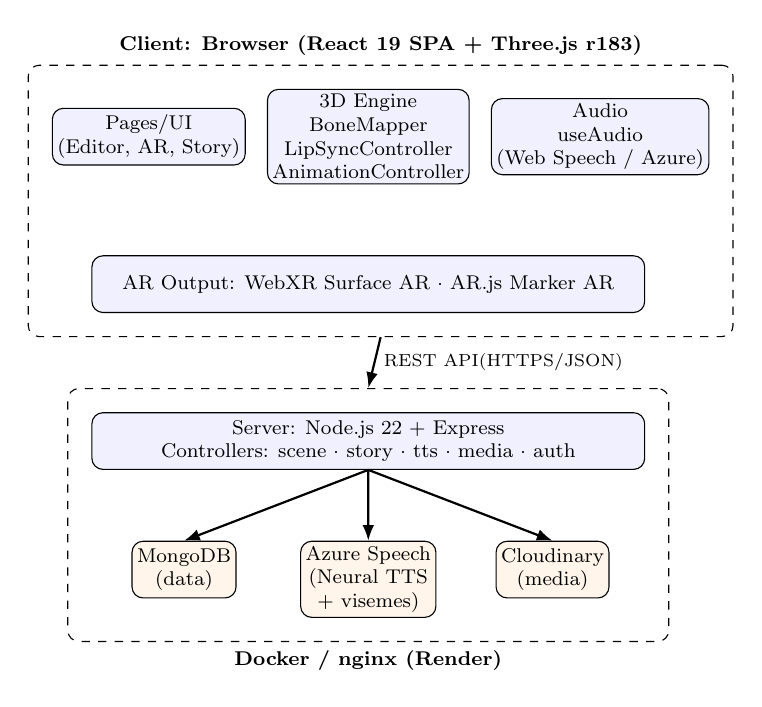
\begin{tikzpicture}[
      scale=0.9, transform shape,
      font=\footnotesize,
      node distance=3mm and 3mm,
      box/.style={draw, rounded corners, align=center, minimum height=8mm, inner sep=2pt, fill=blue!6},
      ext/.style={draw, rounded corners, align=center, minimum height=8mm, inner sep=2pt, fill=orange!8},
      grp/.style={draw, dashed, rounded corners, inner sep=3mm},
      arr/.style={-{Latex[length=2mm]}, thick},
    ]
    % Client layer
    \node[box] (ui) {Pages/UI\\(Editor, AR, Story)};
    \node[box, right=of ui] (engine) {3D Engine\\BoneMapper\\LipSyncController\\AnimationController};
    \node[box, right=of engine] (audio) {Audio\\useAudio\\(Web Speech / Azure)};

    \node[box, below=10mm of engine, minimum width=7.8cm] (ar)
      {AR Output: WebXR Surface AR · AR.js Marker AR};

    \begin{scope}[on background layer]
      \node[grp, fit=(ui)(engine)(audio)(ar),
            label={[font=\footnotesize\bfseries]above:Client: Browser (React 19 SPA + Three.js r183)}]
            (client) {};
    \end{scope}

    % Server layer
    \node[box, below=14mm of ar, minimum width=7.8cm] (server)
      {Server: Node.js 22 + Express\\Controllers: scene · story · tts · media · auth};

    % External services
    \node[ext, below=10mm of server, xshift=-2.6cm] (mongo) {MongoDB\\(data)};
    \node[ext, below=10mm of server] (azure) {Azure Speech\\(Neural TTS\\+ visemes)};
    \node[ext, below=10mm of server, xshift=2.6cm] (cloud) {Cloudinary\\(media)};

    \begin{scope}[on background layer]
      \node[grp, fit=(server)(mongo)(azure)(cloud),
            label={[font=\footnotesize\bfseries]below:Docker / nginx (Render)}]
            (deploy) {};
    \end{scope}

    % Connections
    \draw[arr] (client.south) -- (deploy.north)
      node[midway, right, font=\scriptsize] {REST API\\(HTTPS/JSON)};
    \draw[arr] (server.south) -- (mongo.north);
    \draw[arr] (server.south) -- (azure.north);
    \draw[arr] (server.south) -- (cloud.north);
  \end{tikzpicture}
  \caption{Overall ContAR architecture: the client-side React SPA hosts the 3D
    modules (BoneMapper, LipSyncController, AnimationController) and the audio
    module, communicating via a REST API with the Node.js/Express backend,
    which integrates MongoDB, Azure Speech, and Cloudinary, all running in
    Docker/nginx containers.}
  \label{fig:arquitetura}
\end{figure}

The complete authoring workflow spans four steps integrated into the same
interface, with no need to switch tools or manage intermediate files:
\begin{enumerate}
  \item \textbf{Create avatar:} Avaturn SDK, CC0 gallery, CharacterStudio,
    VRoid Hub, or direct GLB/VRM upload;
  \item \textbf{Configure narration:} speech text, TTS generation (Azure
    Neural TTS or Web Speech API), pose selection, and lip sync;
  \item \textbf{Assemble the story:} save scenes and organize them into
    sequences with a title and description;
  \item \textbf{Publish in AR:} a public link with WebXR Surface AR
    (markerless) or AR.js Marker AR (printed marker).
\end{enumerate}

Fig.~\ref{fig:telas} presents screenshots of the ContAR interface at the main
steps of the workflow.

\begin{figure*}[htbp]
  \centering
  % ── REPLACE with your actual screenshots ──
  % Example usage with subfigures:
  % \begin{subfigure}[b]{0.32\textwidth}
  %   \includegraphics[width=\textwidth]{figs/tela_editor.png}
  %   \caption{3D editor with pose selector}
  % \end{subfigure}
  % ... etc.
  \fbox{%
    \begin{minipage}{0.30\linewidth}
      \centering\vspace{1.8cm}
      \textbf{(a)} 3D Editor\\pose selector
      \vspace{1.8cm}
    \end{minipage}%
  }
  \hfill
  \fbox{%
    \begin{minipage}{0.30\linewidth}
      \centering\vspace{1.8cm}
      \textbf{(b)} Narration\\setup + TTS
      \vspace{1.8cm}
    \end{minipage}%
  }
  \hfill
  \fbox{%
    \begin{minipage}{0.30\linewidth}
      \centering\vspace{1.8cm}
      \textbf{(c)} Surface AR mode\\(WebXR) with avatar
      \vspace{1.8cm}
    \end{minipage}%
  }
  \caption{ContAR interface: (a) 3D editor with pose selector; (b) narration
    configuration and TTS generation panel; (c) Surface AR mode with the
    narrator positioned on a flat surface. Replace with actual screenshots.}
  \label{fig:telas}
\end{figure*}

The decision to support multiple avatar sources was motivated by the need for
phenotypic representation. Avatars with Afro-descendant, Indigenous, and Asian
features are available in the CC0 galleries and can be created in Avaturn
with configurable skin tone, hair type, and facial features. A teacher who
teaches Afro-Brazilian culture should be able to create a Black virtual
narrator without depending on external 3D artists.

\subsection{Technical Modules}

\subsubsection{BoneMapper: Universal Rig Compatibility}

Avatars from different sources use different bone-naming conventions:
Mixamo/Avaturn uses \texttt{mixamorigHips}; VRM uses \texttt{J\_Bip\_C\_Hips};
CC3 uses \texttt{CC\_Base\_Hip}. BoneMapper automatically identifies the rig
standard through heuristic analysis of bone names and maintains an internal
mapping from canonical names to Three.js object references. This lets
procedural poses and animations operate transparently on any avatar
regardless of its origin, removing one of the main technical barriers
identified by Ruiz et al.~\cite{ruiz2020}.

Fig.~\ref{fig:bonemapper} illustrates the mapping process across the three
supported rig standards.

\begin{figure}[htbp]
  \centering
  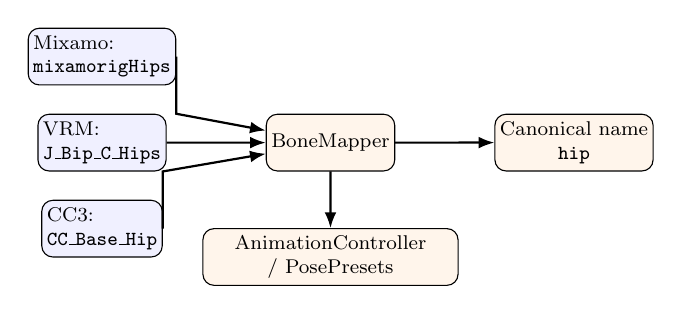
\begin{tikzpicture}[
      scale=0.9, transform shape,
      font=\footnotesize,
      node distance=4mm and 6mm,
      rig/.style={draw, rounded corners, align=left, minimum height=8mm, inner sep=2pt, fill=blue!6},
      core/.style={draw, rounded corners, align=center, minimum height=8mm, inner sep=2pt, fill=orange!8},
      arr/.style={-{Latex[length=2mm]}, thick},
    ]
    \node[rig] (mixamo) {Mixamo:\\\texttt{mixamorigHips}};
    \node[rig, below=of mixamo] (vrm) {VRM:\\\texttt{J\_Bip\_C\_Hips}};
    \node[rig, below=of vrm] (cc3) {CC3:\\\texttt{CC\_Base\_Hip}};

    \node[core, right=14mm of vrm] (mapper) {BoneMapper};
    \node[core, right=14mm of mapper] (canon) {Canonical name\\\texttt{hip}};
    \node[core, below=8mm of mapper, minimum width=3.6cm] (anim) {AnimationController\\/ PosePresets};

    \draw[arr] (mixamo.east) -- (mapper.north -| mixamo.east) -- (mapper);
    \draw[arr] (vrm.east) -- (mapper);
    \draw[arr] (cc3.east) -- (mapper.south -| cc3.east) -- (mapper);
    \draw[arr] (mapper) -- (canon);
    \draw[arr] (mapper) -- (anim);
  \end{tikzpicture}
  \caption{BoneMapper: automatic mapping of bone names from the supported rig
    standards (Mixamo, VRM, CC3) to canonical Three.js names, used by the
    AnimationController and the PosePresets.}
  \label{fig:bonemapper}
\end{figure}

\subsubsection{LipSyncController: Multi-Mode Lip Synchronization}

The LipSyncController operates in two modes: (1)~\textbf{timeline mode}, which
consumes a time-stamped sequence of viseme cues, applied with configurable
crossfade, obtained directly from Azure Neural TTS (IDs~0--21 mapped to
Rhubarb codes~A--X, with 100\,ns precision) or estimated locally from the
speech text when the audio is generated by the Web Speech API or supplied by
the user (recording or upload); and (2)~\textbf{heuristic mode}, which
estimates lip movement in real time from amplitude and frequency analysis of
the audio signal via the Web Audio API, used as a fallback for imported audio
with no corresponding text. The controller automatically discovers the
avatar's speech blend shapes through regular-expression patterns over the
morph target names.

\subsubsection{AnimationController: Procedural Poses and Animations}

The AnimationController manages Three.js's \texttt{AnimationMixer} with
smooth crossfading and implements procedural micro-animations (blinking,
breathing, speaker gestures). The system supports 18 presets: 7~animated
(\textit{idle, walk, walk\_circle, slow\_run, run, dance, speaker}) and
11~static. For VRM avatars, it supports the VRM Animation standard via
\texttt{@pixiv/three-vrm-animation}.

\subsection{Interface and User Experience}

ContAR's interface was designed following progressive-disclosure principles:
basic controls are always visible, while advanced settings are collapsible.
An 11-step guided tour orients the user on first access. The system includes
automatic autosave, internationalization in four languages (PT, EN, ES, FR),
light and dark themes, and a progress bar that indicates the steps still
pending for a complete scene. The speech text can be displayed as a speech
bubble overlaid on the avatar (\textit{bubble}), as a caption at the bottom of
the screen (\textit{subtitle}), or hidden (\textit{none}).

% ──────────────────────────────────────────────────────────────────────────────
\section{ContAR and Anti-Racist Education: A Pedagogical Use Case}

\subsection{Rationale and Motivation}

Law~10.639/2003, the result of the historic struggle of the Black Movement
(\textit{Movimento Negro})~\cite{santos2005}, mandated the teaching of
Afro-Brazilian and African history and culture in Brazilian basic education
schools. More than two decades after its enactment, its implementation
remains uneven, partly due to the scarcity of representative teaching
materials~\cite{araujo2023a,rocha2015}.

Djamila Ribeiro~\cite{ribeiro2019} argues that denying Black people their own
history and the possibility of seeing themselves represented in spaces of
knowledge is a form of symbolic violence that is perpetuated daily. Jeferson
Tenório, in \textit{O Avesso da Pele}~\cite{tenorio2020}, builds a narrative
in which the Black teacher protagonist is confronted, in every class, with his
own absence from the teaching materials. This resistance manifests
concretely: in 2024, the book was censored in schools across three Brazilian
states, under a mistaken justification about its content~\cite{g1_2024}.
These perspectives call on us to understand ContAR not merely as a technical
tool, but as an instrument of educational policy: by allowing any teacher to
create a Black virtual narrator who tells the story of Zumbi dos Palmares,
Carolina Maria de Jesus, or Machado de Assis, the platform democratizes the
production of pedagogical memory.

\subsection{Example Story: \textit{Dandara dos Palmares}}

To illustrate ContAR's pedagogical potential in the anti-racist context, the
story \textit{Dandara dos Palmares} was developed for 5th-grade elementary
school students and created entirely on the platform without external
technical expertise. Fig.~\ref{fig:dandara} presents captures of the three
scenes of this story in AR mode.

\begin{figure}[htbp]
  \centering
  \fbox{%
    \begin{minipage}{0.9\columnwidth}
      \centering
      \vspace{1.8cm}
      \textbf{[Fig. 4. ``Dandara dos Palmares'' story]}\\[4pt]
      \small
      Scene 1: Dandara avatar, \textit{speaker} pose\\
      Scene 2: Dandara avatar, \textit{walk\_circle} pose\\
      Scene 3: Dandara avatar, \textit{neutral} pose + text bubble\\[4pt]
      Publication: AR.js Marker AR via public link
      \vspace{1.8cm}
    \end{minipage}%
  }
  \caption{\textit{Dandara dos Palmares} story in AR.js Marker AR mode: three
    scenes with a phenotypically diverse virtual narrator, Portuguese TTS,
    and lip sync. Replace with actual platform screenshots.}
  \label{fig:dandara}
\end{figure}

\textbf{Scene~1: ``Who was Dandara?''} Avatar: a Black woman with voluminous
curly hair, created in Avaturn with dark skin tone and clothing inspired by
17th-century \textit{quilombola} (maroon community) attire. Pose:
\textit{speaker}. Speech (Azure TTS, Brazilian Portuguese female voice,
translated from Portuguese): \textit{``My name is Dandara. I was a warrior, a
mother, and a leader. I lived in the Quilombo dos Palmares, a land of freedom
built by men and women who refused to be enslaved. Our history does not begin
in chains. It begins in kingdoms.''}

\textbf{Scene~2: ``The Quilombo dos Palmares''} Same avatar, \textit{walk\_circle}
pose. Speech: \textit{``Palmares was a nation of more than twenty thousand
free people. My companion Zumbi was the warrior leader. But I fought too. No
history of Palmares is complete without speaking of its women.''}

\textbf{Scene~3: ``Why remember?''} \textit{Neutral} pose, text bubble enabled.
Speech: \textit{``Today, November 20th, is Black Awareness Day. It's not a day
of sadness: it's a day of memory and pride. I am Dandara. And my story is
part of yours.''}

The story was published in AR.js Marker AR mode, generating a public link
that can be printed in educational booklets. The complete workflow, from
avatar creation to publication, was completed in approximately 25~minutes,
with no code written.

\subsection{Pedagogical Implications and Design Decisions}

ContAR's design decisions are pedagogically motivated: (i) support for
avatars with African and Afro-Brazilian phenotypes is a precondition for
anti-racist education; (ii) Brazilian Portuguese voice synthesis lets the
virtual narrator sound like someone from the student's own community;
(iii) sequential story composition allows narratives to be structured with a
beginning, middle, and end, a format recognized as more effective for
memorization and engagement~\cite{fonnet2021}; (iv) publication via printed
marker is especially relevant for schools with poor connectivity.

These decisions directly echo the principles of Silva et
al.~\cite{silva2023}: a guided, code-free workflow, contextual customization,
and integration between creation and publication.

% ──────────────────────────────────────────────────────────────────────────────
\section{Evaluation Methodology}

\subsection{Expert Walkthrough}

The Expert Walkthrough is a formative evaluation technique in which experts
systematically walk through a system's tasks, identifying problems according
to established heuristics~\cite{nielsen1994}. It requires only 3--5 evaluators
to detect approximately 75\% of usability problems, making it suitable for
the development stage ContAR is currently in.

\subsection{Participants}

Three experts with complementary profiles were recruited:

\begin{itemize}
  \item \textbf{E1}: expert in Human-Computer Interaction and
    Augmented/Virtual Reality, with experience in computer systems and
    interface evaluation.
  \item \textbf{E2}: expert in anti-racist education and racial literacy,
    involved in teacher-training courses on anti-racist perspectives in
    Pernambuco~\cite{araujo2023a}.
  \item \textbf{E3}: expert in educational Augmented Reality and content
    authoring, with publications on AR-authoring design principles that
    underpin ContAR~\cite{silva2022,silva2023}.
\end{itemize}

\subsection{Protocol and Tasks}

Sessions were conducted individually, remotely, using a Think Aloud protocol.
Each session had an estimated average duration of 60--90 minutes. The experts
performed five tasks covering the full authoring workflow:

\begin{itemize}
  \item \textbf{T1. Create avatar}: access the platform, create or import an
    avatar, and view it in the 3D editor.
  \item \textbf{T2. Configure speech and generate voice}: type a text,
    select a voice, and generate audio with lip synchronization.
  \item \textbf{T3. Set pose and save the scene}: select a pose, name and
    save the scene.
  \item \textbf{T4. Compose and publish a story}: add scenes to a story and
    obtain the public link.
  \item \textbf{T5. View in AR}: access the link on a phone and play the
    story in Surface AR (WebXR) or Marker AR (AR.js).
\end{itemize}

Three methodological decisions should be noted: (i)~the 11-step guided tour
was deliberately turned off in all sessions, so the results reflect the
worst-case scenario (zero onboarding); (ii)~bug fixes between sessions were
allowed (by formal agreement with E1), but UX/UI changes were not applied,
preserving data comparability; and (iii)~during E3's session, the researcher
actively intervened in T4, explaining the correct scene/story workflow before
requesting a second attempt --- a one-off departure from the pure Think Aloud
protocol that should be taken into account when interpreting the data for
that task. The mapping of identified problems to Nielsen's heuristics was
performed by the researcher in the post-session analysis, based on the
qualitative reports.

\subsection{Heuristics and Instruments}

The analysis used Nielsen's 10 heuristics~\cite{nielsen1994}, complemented by
three XR criteria from Gabbard and Swan~\cite{gabbard2008}: (XR1) stability
and anchoring of virtual objects; (XR2) tracking and AR-state feedback; (XR3)
ergonomics of interaction in a mobile setting. The severity of each problem
was rated on Nielsen's scale (0--4).

After the sessions, the experts completed the System Usability Scale (SUS)
questionnaire~\cite{brooke1996}, which produces a score from 0 to 100 (above
68: above average; above 80: \textit{good}; above 90: \textit{excellent}).

% ──────────────────────────────────────────────────────────────────────────────
\section{Results}

\subsection{SUS Score}

The mean System Usability Scale score was \textbf{77.5} points (SD~=~15.2),
rated ``\textbf{above average}'' according to Bangor et
al.~\cite{bangor2009}. Table~\ref{tab:sus} presents the individual scores.

\begin{table}[htbp]
\caption{SUS scores by expert}
\label{tab:sus}
\begin{center}
\renewcommand{\arraystretch}{1.2}
\begin{tabular}{|c|l|c|}
\hline
\textbf{Expert} & \textbf{Profile} & \textbf{SUS} \\
\hline
E1 & HCI / AR and VR  & 85.0 \\
E2 & Anti-Racist Education & 60.0 \\
E3 & Educational AR / Authoring & 87.5 \\
\hline
\textbf{Mean (SD = 15.2)} & & \textbf{77.5} \\
\hline
\end{tabular}
\end{center}
\end{table}

\subsection{Identified Problems}

A total of \textbf{15} usability problems were catalogued across the
sessions. Table~\ref{tab:heuristicas} summarizes the distribution by
violated heuristic and mean severity.

\begin{table}[htbp]
\caption{Distribution of problems by heuristic and severity}
\label{tab:heuristicas}
\begin{center}
\renewcommand{\arraystretch}{1.2}
\begin{tabular}{|l|c|c|}
\hline
\textbf{Heuristic} & \textbf{Occ.} & \textbf{Mean Sev.} \\
\hline
H1. Visibility of system status    & 3 & 3.3 \\
H2. Match between system and world & 3 & 2.3 \\
H3. User control and freedom       & 2 & 2.5 \\
H5. Error prevention               & 3 & 3.0 \\
H6. Recognition rather than recall & 1 & 4.0 \\
H7. Flexibility and efficiency     & 1 & 3.0 \\
H9. Error recovery                 & 1 & 4.0 \\
XR1. Anchoring of virtual objects  & 1 & 4.0 \\
\hline
\textbf{Total} & \textbf{15} & \textbf{3.1} \\
\hline
\end{tabular}
\end{center}
\end{table}

\subsection{Qualitative Analysis}

All quotes below were originally given in Portuguese and are translated by
the authors. The analysis of verbalizations recorded during the Think Aloud
sessions revealed consistent patterns across experts.

\textbf{Strengths.} Avatar creation was considered intuitive (E3: ``I found
it quite intuitive, it wouldn't even need that much guidance''), and E1 noted
that ``in 2~minutes I could already see the tool's full potential.'' E1
spontaneously validated the anti-racist use case by creating, without
instruction, an ``anti-racist version'' of \textit{The Little Prince}. The
overall viability was summarized by E1: ``it's not perfect, but it's much
better than not having it.'' E2, despite the lower SUS score, stated that she
``would use this to enliven educational processes.''

\textbf{Opportunities for improvement.} Confusion between ``save scene'' and
``add scene to story'' was the most recurring finding (4/4 sessions). The
TTS $\to$ lip-sync sequence was considered by E3 the ``least intuitive'' step
of all. E3 also saved two of four scenes without generating audio, revealing
a lack of validation in the flow (``you know I didn't generate its speech? I
remember clicking on all of them''). Regarding representation, E3 reported
that the catalog did not allow her to represent her pregnancy, and E1
observed that ``the tool's limit is still \textit{moreno} [medium-brown skin
tone]'' for skin tones, broadening the discussion beyond the racial axis.

% ──────────────────────────────────────────────────────────────────────────────
\section{Discussion}

\subsection{Comparison with the Prior Benchmark}

The preliminary exploratory study conducted by the authors found that the
fragmented ecosystem requires multiple transitions between platforms to
complete the authoring workflow. ContAR eliminates this fragmentation by
integrating the entire workflow into a single interface. The mean SUS score
of~77.5 points confirms that this integration does not compromise usability,
reaching the \textit{above average} level and surpassing the benchmark of the
standalone tools assessed in that survey. However, the high standard
deviation (SD~=~15.2) reveals that the perception of usability is not uniform
across profiles: E2, whose background is in education and racial literacy
(with no prior experience with 3D interfaces), scored 60.0 points, while E1
and E3, with backgrounds in computing and AR, converged around 86~points
(85.0 and 87.5). This disparity suggests that ContAR already serves users
with prior technological familiarity well, but requires additional onboarding
effort for the primary target audience --- basic-education teachers without
technical training. E2's observation that ``the person using it might think
the problem is with them, not with the system'' reinforces the need for the
platform to communicate more clearly that workflow errors are interface
limitations, not user failures.

\subsection{Technical Validation of the Modules}

BoneMapper demonstrated compatibility with the four rig standards tested
(Mixamo, VRM, CC3, and generic) with no manual configuration, confirming
that name-based mapping heuristics are sufficient for most avatars on
no-code platforms. The Azure viseme-timeline lip-sync mode produced
synchronization perceived as natural by the experts, while the heuristic
mode was considered satisfactory for imported audio.

\subsection{Study Limitations}

The Expert Walkthrough does not replace testing with the primary target
audience, basic-education teachers; an evaluation with end users may reveal
additional barriers related to technological familiarity. WebXR support for
Surface AR varies across devices and browsers, especially across Safari
versions on iOS. E1's session may have been slightly influenced by his having
observed a fragment of E2's session, and the researcher's active intervention
in E3's session (T4) limits the comparability of that portion of the data.

Phenotypic representation remains limited by the Avaturn SDK catalog:
insufficient granularity at the extreme skin tones (E1: ``the tool's limit is
still \textit{moreno}''), an interface that is always in English (no language
parameter in the SDK), and a lack of body diversity beyond weight --- E3,
pregnant during the evaluation, reported that ``the representation is
so-so.''

Finally, the anti-racist use case, although theoretically grounded, has not
yet been empirically evaluated with students and teachers in a real-world
context.

% ──────────────────────────────────────────────────────────────────────────────
\section{Conclusion}

This paper presented ContAR, a no-code web platform for authoring 3D virtual
narrators in educational WebAR, and its usability evaluation via an Expert
Walkthrough. The contributions are fourfold: (i)~\textbf{architectural}:
integration of avatar creation, viseme-based TTS, story composition, and
WebAR publication into a single in-browser workflow; (ii)~\textbf{technical}:
BoneMapper with universal rig compatibility, a LipSyncController with
timeline and heuristic modes, and support for the VRM Animation standard;
(iii)~\textbf{evaluative}: an Expert Walkthrough protocol combining Nielsen +
XR heuristics and SUS; and (iv)~\textbf{pedagogical}: the proposal and
demonstration of an anti-racist use case aligned with Law~10.639/2003.

ContAR confirms that it is possible to implement an integrated, in-browser
educational WebAR authoring ecosystem, reducing the fragmentation identified
in the preliminary study and making the complete workflow accessible to
users without technical training. More than that, this work demonstrates
that XR authoring tools can be designed with an explicit pedagogical agenda,
placing technology at the service of equity and representation in Brazilian
education.

Future work includes: (i) evaluation with basic-education teachers,
especially in schools implementing anti-racist programs; (ii) integration of
VRM facial expressions and eye-tracking; (iii) incorporation of an LLM to
create narrators that respond to student questions; and (iv) application in
a real-world teacher-training context, in partnership with Voxar~Labs/CIn-UFPE.

The source code is available at \url{https://github.com/jorgelcff/contar}.

% ──────────────────────────────────────────────────────────────────────────────
\begin{thebibliography}{00}

\bibitem{fonnet2021}
A.~Fonnet and Y.~Prie, ``Survey of augmented reality for education,''
\textit{Computers \& Education}, vol.~159, p.~104005, 2021.

\bibitem{munoz2021}
J.~A.~Munoz-Cristóbal et al., ``Augmented reality in education: A systematic
review,'' \textit{Educational Technology Research and Development}, vol.~69,
pp.~1--28, 2021.

\bibitem{koutsabasis2021}
P.~Koutsabasis and S.~Vosinakis, ``Web-based augmented reality: A review of
tools, features and applications,'' \textit{Multimedia Tools and Applications},
vol.~80, pp.~1--34, 2021.

\bibitem{ibge2022}
IBGE, \textit{Censo Demográfico 2022: Panorama} [2022 Demographic Census:
Overview]. Rio de Janeiro: Instituto Brasileiro de Geografia e Estatística
(Brazilian Institute of Geography and Statistics), 2023.

\bibitem{ribeiro2019}
D.~Ribeiro, \textit{Pequeno Manual Antirracista} [Small Anti-Racist
Handbook]. São Paulo: Companhia das Letras, 2019.

\bibitem{ribeiro2018}
D.~Ribeiro, \textit{Quem tem medo do feminismo negro?} [Who's Afraid of
Black Feminism?] São Paulo: Companhia das Letras, 2018.

\bibitem{tenorio2020}
J.~Tenório, \textit{O Avesso da Pele} [The Reverse Side of the Skin]. São
Paulo: Companhia das Letras, 2020.

\bibitem{g1_2024}
G1 Educação, ```O avesso da pele', livro que debate racismo, é censurado em
escolas de 3 estados por reação equivocada ao conteúdo, alertam
especialistas'' [``The Reverse Side of the Skin,'' a book that discusses
racism, is censored in schools in 3 states due to a mistaken reaction to its
content, experts warn], \textit{G1}, Mar. 2024. [Online]. Available:
\url{https://g1.globo.com/educacao/noticia/2024/03/08/o-avesso-da-pele-livro-que-debate-racismo-e-censurado-em-escolas-de-3-estados-por-reacao-equivocada-ao-conteudo-alertam-especialistas.ghtml}

\bibitem{santos2005}
S.~A.~dos Santos, ``A Lei no. 10.639/03 como fruto da luta anti-racista do
Movimento Negro'' [Law 10.639/03 as a result of the Black Movement's
anti-racist struggle], in \textit{Educação Anti-Racista: Caminhos Abertos
pela Lei Federal no. 10.639/03} [Anti-Racist Education: Paths Opened by
Federal Law 10.639/03]. Brasília: Ministério da Educação, Secretaria de
Educação Continuada, Alfabetização e Diversidade, 2005.

\bibitem{rocha2015}
L.~F.~R.~Rocha, ``A implementação da Lei 10.639/2003 na Rede Federal de
Educação Profissional, Científica e Tecnológica'' [The implementation of
Law 10.639/2003 in the Federal Network of Professional, Scientific and
Technological Education], Master's thesis (Education), Universidade Federal
de Ouro Preto (UFOP), Ouro Preto, 2015.

\bibitem{araujo2023a}
G.~J.~Ferreira de Araújo, ``Profissionais de educação recebem curso de
letramento racial e educação antirracista'' [Education professionals
receive a racial-literacy and anti-racist education course], Radio
interview/program, 2023.

\bibitem{araujo2023b}
G.~J.~Ferreira de Araújo, ``UPE realiza curso sobre letramento racial e
educação antirracista em Petrolina'' [UPE holds a racial-literacy and
anti-racist education course in Petrolina], Radio interview/program, 2023.

\bibitem{araujo2023c}
G.~J.~Ferreira de Araújo, ``Letramento racial e educação antirracista são
temas de curso no Vale do SF'' [Racial literacy and anti-racist education
are the themes of a course in the São Francisco Valley], Radio
interview/program, 2023.

\bibitem{silva2020}
M.~M.~O.~Silva et al., ``Why don't we see more of augmented reality in
schools?'' in \textit{Proc. IEEE ISMAR-Adjunct}, 2020, pp.~138--143.

\bibitem{silva2022}
M.~M.~O.~Silva, ``Development of design principles to author AR in education
based on teacher's perspectives,'' Ph.D.\ dissertation, Centro de Informática,
UFPE, Recife, 2022.

\bibitem{silva2023}
M.~M.~O.~Silva et al., ``Development of design principles for AR authoring tools
for education based on teacher's perspectives,'' \textit{IEEE Transactions on
Learning Technologies}, vol.~16, pp.~1--14, 2023.

\bibitem{ruiz2020}
J.~Ruiz and Y.~Li, ``Designing for augmented reality beginners,'' \textit{IEEE
Computer Graphics and Applications}, vol.~40, no.~4, pp.~72--80, 2020.

\bibitem{fernandes2025}
R.~Fernandes and I.~F.~Silveira, ``Daz Studio to VRM pipeline: a discussion on
the use of realistic VRM 3D models in upper body motion tracking,'' in
\textit{Anais Estendidos do SVR 2025}, Porto Alegre: SBC, 2025, pp.~23--29.
DOI: 10.5753/svr\_estendido.2025.15640.

\bibitem{santos2025}
S.~E.~F.~Santos et al., ``Teacher representations in immersive environments
through holograms: A narrative review on the perspectives and challenges,'' in
\textit{Proc. SVR 2025}, Porto Alegre: SBC, 2025.
DOI: 10.1109/SVR67689.2025.11338574.

\bibitem{nielsen1994}
J.~Nielsen, \textit{Usability Engineering}. Boston: Academic Press, 1994.

\bibitem{gabbard2008}
J.~L.~Gabbard and J.~E.~Swan, ``Usability engineering for augmented reality,''
\textit{IEEE Trans. Vis. Comput. Graphics}, vol.~14, no.~3, pp.~513--525, 2008.

\bibitem{brooke1996}
J.~Brooke, ``SUS: A quick and dirty usability scale,'' in \textit{Usability
Evaluation in Industry}, P.~Jordan et al., Eds. London: Taylor \& Francis,
1996, pp.~189--194.

\bibitem{bangor2009}
A.~Bangor, P.~Kortum, and J.~Miller, ``Determining what individual SUS scores
mean: Adding an adjective rating scale,'' \textit{J. Usability Studies},
vol.~4, no.~3, pp.~114--123, 2009.

\bibitem{milgram1994}
P.~Milgram and F.~Kishino, ``A taxonomy of mixed reality visual displays,''
\textit{IEICE Trans. Inf. Syst.}, vol.~E77-D, no.~12, pp.~1321--1329, 1994.

\bibitem{azuma1997}
R.~T.~Azuma, ``A survey of augmented reality,'' \textit{Presence: Teleoperators
and Virtual Environments}, vol.~6, no.~4, pp.~355--385, 1997.

\end{thebibliography}

\end{document}
